\chapter{Metodologia}\label{cap:metodologia}

\todo[inline]{Revisar após conclusão dos experimentos}

Neste capítulo é descrita a sequência de etapas que serão realizadas neste trabalho para que os objetivos de pesquisa sejam alcançados.

Em imagens aéreas como as utilizadas neste trabalho, é comum que os elementos que indicam presença humana sejam relativamente grandes (pista de pouso, estradas, clareiras, etc.), podendo ser definidas como uma região durante a segmentação da imagem. Mas muitas vezes, por outro lado, os objetos ou sinais são pequenos demais para serem encontrados no processo de segmentação (carros, barcos, cabanas, etc.), o que torna interessante um nível adicional de classificação da imagem: uma que possa inspecionar o interior das regiões encontradas durante a segmentação e possa procurar por elementos antrópicos mais sutis na imagem.

Por este motivo, a arquitetura para a solução proposta prevê uma etapa de segmentação das imagens, seguida por dois níveis de classificação: um responsável pela determinação do tipo de cada região encontrada na segmentação; e um outro responsável pela busca de elementos antrópicos no interior destas mesmas regiões. A arquitetura geral da solução pode ser vista na figura \ref{fig:metDiagrama}.

\begin{figure}[h]
    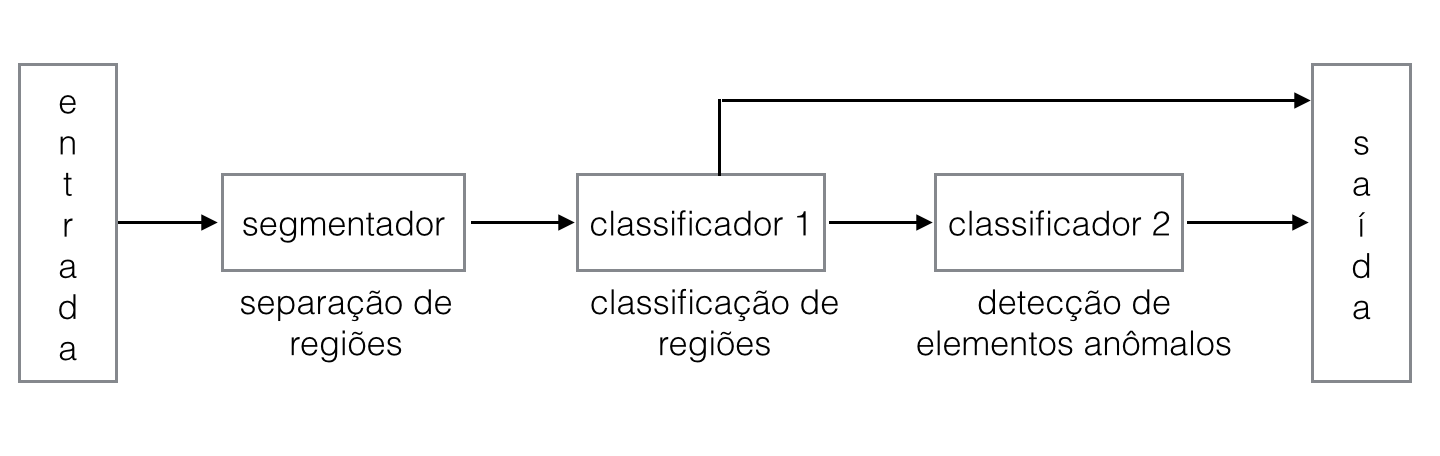
\includegraphics[width=\textwidth]{imgs/arquitetura}
    \caption{Arquitetura da solução a ser desenvolvida para detecção de elementos antrópicos em imagens aéreas da floresta amazônica}
    \label{fig:metDiagrama}
\end{figure}

A primeira etapa do trabalho é a segmentação das imagens por tipo de terreno. Os métodos de segmentação de imagens considerados estado-da-arte serão aplicados à uma parte da base de imagens aéreas da floresta amazônica. Esta porção da base de imagens será manualmente segmentada por seres humanos e servirá de base de comparação para a segmentação realizada pelos métodos experimentados. Esta etapa deve determinar o método de segmentação com melhores resultados, a ser utilizado na solução descrita pelo trabalho.

Posteriormente, as regiões encontradas na segmentação das imagens devem ter suas características extraídas para serem classificadas dentre diversas classes: floresta, vegetação rasteira, clareira, corpos d'água e elementos antrópicos. É nesta etapa que se dará o primeiro nível de classificação. Serão utilizados os métodos descritos na seção \ref{sec:trClassificacao}. O resultado da classificação dos segmentos por cada método será comparado à uma classificação realizada por seres humanos, permitindo que os métodos de aprendizagem supervisionados sejam utilizados. As regiões classificadas como "elementos antrópicos" serão prontamente consideradas objetos de interesse. As demais regiões serão classificadas de acordo com seu tipo de terreno pertinente e serão investigadas com mais detalhes na próxima etapa.

A última etapa de classificação consiste em utilizar modelos de aprendizado específicos para cada tipo de terreno, para detectar elementos antrópicos que não foram encontrados na etapa de segmentação, normalmente pequenos demais para serem definidos como uma região \textit{per se}, e que estão contidos em regiões maiores. Cada tipo de terreno possuirá um modelo de classificação específico, podendo se utilizar de um vetor de características diferente dos demais terrenos, a fim de otimizar a precisão na detecção dos objetos de interesse. Nesta etapa, diversos classificadores serão treinados e testados para cada tipo de terreno e seus resultados serão comparados com uma classificação manual feita por um especialista. Nesta etapa serão explorados classificadores unários e multi-classe a fim de obter o melhor resultado na detecção dos elementos antrópicos do segmento de imagem e um classificador, com seus parâmetros e vetor de características, será selecionado para cada tipo de terreno.

Por fim, unindo a saída do primeiro nível de classificação, onde regiões de "elementos antrópicos" podem ser encontradas, com a saída do segundo nível, onde os objetos de interesse serão procurados no interior das demais regiões, teremos uma saída única, apontando as regiões de uma imagem que possuam objetos de interesse na problemática em questão.

As sucessivas validações e comparações com a segmentação e classificação manual feita por seres humanos é importante para diminuir o erro em cada etapa, visto que imprecisões em um dos passos tendem a propagar o erro nos passos seguintes. Se tomarmos como exemplo o princípio da solução, uma segmentação inadequada de uma imagem pode dificultar o primeiro nível de classificação, responsável pela classificação do tipo de região encontrada.

O próximo capítulo descreve os experimentos realizados e discute os resultados encontrados.